\documentclass[12pt]{article}
\setlength{\oddsidemargin}{0in}
\setlength{\evensidemargin}{0in}
\setlength{\textwidth}{6.5in}
\setlength{\parindent}{0in}
\setlength{\parskip}{\baselineskip}
\usepackage{amsmath,amsfonts,amssymb}
\usepackage{graphicx}
\usepackage{enumitem}
\usepackage[]{algorithmicx}
\usepackage{amsthm}
\usepackage{fancyhdr}
\pagestyle{fancy}
\setlength{\headsep}{36pt}
\usepackage{tkz-berge}
\usetikzlibrary{positioning, automata}

\usepackage{hyperref}

\theoremstyle{remark}
\newtheorem*{solution}{Solution}

\newcommand{\makenonemptybox}[2]{%
%\par\nobreak\vspace{\ht\strutbox}\noindent
\item[]
\fbox{% added -2\fboxrule to specified width to avoid overfull hboxes
% and removed the -2\fboxsep from height specification (image not updated)
% because in MWE 2cm is should be height of contents excluding sep and frame
\parbox[c][#1][t]{\dimexpr\linewidth-2\fboxsep-2\fboxrule}{
  \hrule width \hsize height 0pt
  #2
 }%
}%
\par\vspace{\ht\strutbox}
}
\makeatother

\begin{document}

\lhead{{\bf CSCI 3104, Algorithms \\ Problem Set 7a (14 points)} }
\rhead{Name: \fbox{Michael Rogers} \\ ID: \fbox{105667404} \\ {\bf Profs.\ Hoenigman \& Agrawal\\ Fall 2019, CU-Boulder}}
\renewcommand{\headrulewidth}{0.5pt}

\phantom{Test}

\begin{small}
\textit{Advice 1}:\ For every problem in this class, you must justify your answer:\ show how you arrived at it and why it is correct. If there are assumptions you need to make along the way, state those clearly.
\vspace{-3mm} 

\textit{Advice 2}:\ Verbal reasoning is typically insufficient for full credit. Instead, write a logical argument, in the style of a mathematical proof.\\
\vspace{-3mm} 

\textbf{Instructions for submitting your solution}:
\vspace{-5mm} 

\begin{itemize}
	\item The solutions \textbf{should be typed} and we cannot accept hand-written solutions. \href{http://ece.uprm.edu/~caceros/latex/introduction.pdf}{Here's a short intro to Latex.}
	\item You should submit your work through \href{https://www.gradescope.com/courses/59294}{\textbf{Gradescope}} only.
	\item If you don't have an account on it, sign up for one using your CU email. You should have gotten an email to sign up. If your name based CU email doesn't work, try the identikey@colorado.edu version. 
	\item Gradescope will only accept \textbf{.pdf} files (except for code files that should be submitted separately on Gradescope if a problem set has them) and \textbf{try to fit your work in the box provided}. 
	\item You cannot submit a pdf which has less pages than what we provided you as Gradescope won't allow it. 
\end{itemize}
\vspace{-4mm} 
\end{small}

\hrulefill
\pagebreak

\begin{enumerate}

    \item (1 pt) Provide a one-sentence description of each of the components of a divide and conquer algorithm.
    
    \begin{solution}
    Divide: Break problems into several smaller instances of the same problem with the same attributes. \\ \\
Conquer: If smaller instance is trivial, solve it. Otherwise, divide the array again. \\ \\
Combine: Combine results for smaller problems into solution for the larger problem.
    \end{solution}
    
    \item (3 pts) Use the array $A=[2,5,1,6,7,9,3]$ for the following questions
    \begin{enumerate}
        \item (1 pt) What is the value of the pivot in the call $partition(A,0,6)$?
        
        \begin{solution}
        Pivot = 3, assuming we are using the technique presented in class which takes the pivot to be the last element in the array.
        \end{solution}
        
        \item (1 pt) What is the index of that pivot value at the end of that call to $partition()$?
        
        \begin{solution}
        Index of Pivot = 2. All elements to the left of the pivot are less than the pivot and all elements to the right are greater than the pivot.
        \end{solution}
        
        \item (1 pt) On the next recursive call to Quicksort, what sub-array does $partition()$ evaluate?
        
        \begin{solution}
        \{2,1\}, or the left sub-array of the pivot.
        \end{solution}
        
    \end{enumerate}
	\item (4 pts) Draw the tree of recursive calls that Quicksort makes to sort the list \\${E,X,A,M,P,L,E}$ in alphabetical order. Use the last element in the sub-list in each recursive call as the pivot.
	
	\begin{solution}
        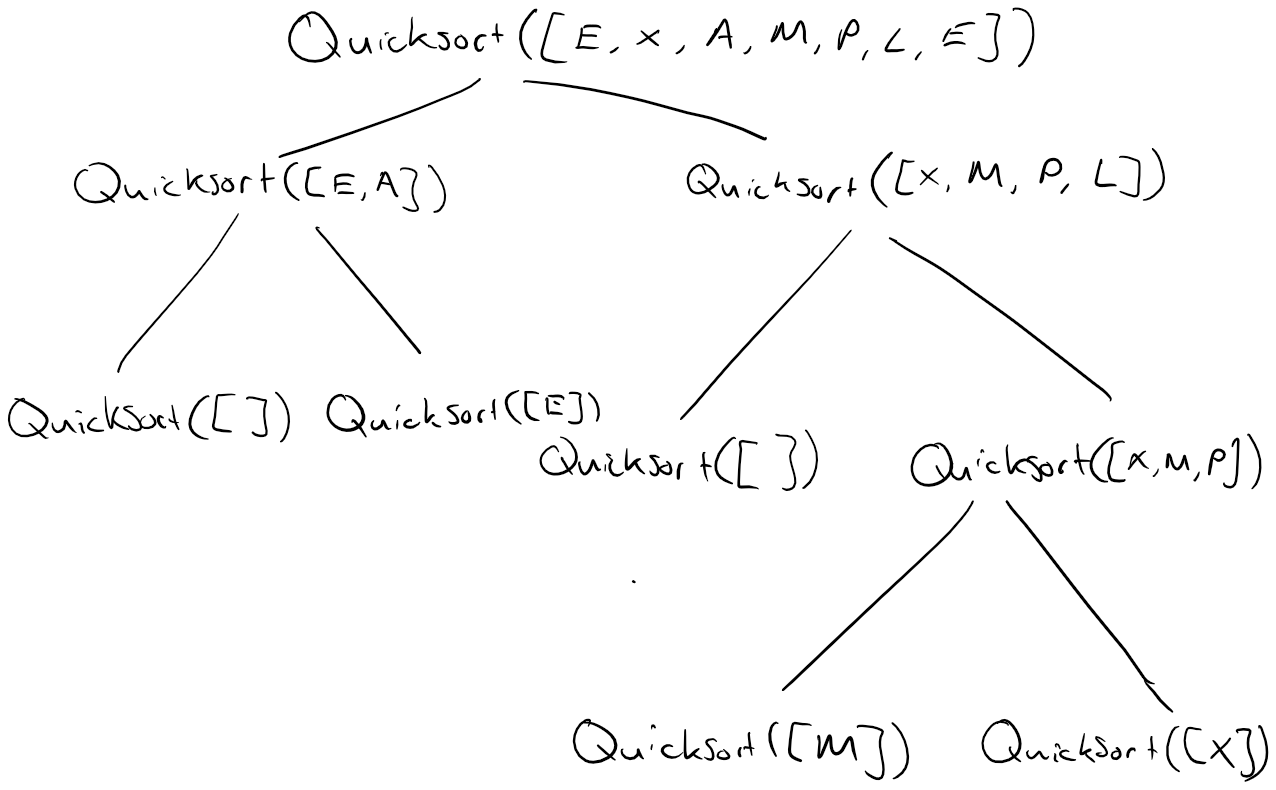
\includegraphics[scale=0.5]{PS7a-Q3.png}
    \end{solution}
	

    \item (6 pts) You are given a collection of $n$ bottles of different widths and $n$ lids of different widths and you need to find which lid goes with which bottle. You can compare a lid to a bottle, from which you can determine if the lid is larger than the bottle, smaller than the bottle, or the correct size. However, there is no way to compare the bottles or the lids directly to each other, i.e. you can't compare lids to lids or bottles to bottles. Design an algorithm for this problem with an average-case efficiency of $\Theta(nlgn)$
    
    \begin{solution}
        Assuming every bottle has a lid and no two lids or bottles are the same size:\\
Spose' B = $\{bottle_{1}, bottle_{2},  ... , bottle_{n}\}$, \\
L = $\{lid_1, lid_2, ... , lid_n\}$
In order for these two arrays to be sorted correctly, there must be an attribute of each matching bottle and lid that must be the same. Therefore we can use the pivot of one array on the other to acheive the same result because the two arrays must contain the same values in different orders. This will allow us to use quicksort without comparing bottles to bottles or lids to lids.
\begin{verbatim}
BottleMatch(B, L):
   Quicksortesque(A, B, p, r):
      if p <  r: // If low index is less than the high index
         // Value of the last element of the array B to use for partition of A.
         A-piv = partition(A, p, r, B[r])
         // Partition B by same partition value as A 
         partition(B, p, r, A[A-piv])
        
         Quicksortesque(A, B , p, r - 1) //Sub-array left of pivot
         Quicksortesque(A, B , p + 1, r) //Sub-array right of pivot

   Quicksortesque(B, L, 0, len(B)) // len(B) = len(L)
   
   return B, L
\end{verbatim}
partition() takes in the two arrays and finds the partition of the first array by the last values of the second. Once it finds this partition value it partitions the second array by the same value as the first. After it partitions both of the arrays, it runs quicksort on both arrays making the corresponding lids and bottles have the same index in their respective arrays. The runtime of this algorithm would be O($2n\log(n)$) because we run quicksort on both arrays, which equals O($n\log(n)$).
    \end{solution}
    
\end{enumerate}


\end{document}


